%%%%%%%%%%% Single Column %%%%%%%%%%%%%%%%%
\documentclass[1p, number, sort&compress,table, 11pt]{elsarticle}
%%%%%%%%%% Double Column %%%%%%%%%%%%%%%%%%%
%\documentclass[preprint, 3p, twocolumn, number, sort&compress,table]{elsarticle}
%%%%%%%%%%%%%%%%%%%%%%%%%%%%%%%%%%%%%%%%%%%%%   

\usepackage{styles/mainStyles}   % Set for for extra stylings
\usepackage{helvet}
\renewcommand{\familydefault}{\sfdefault}

% hyperlinking is set to color blue.
% \autoref is currently set to cross references figures as 'Fig. 1', and equations as 'Eq.1'. 
%This can be changed
%%%%%%%%%%%%%%%%%%%%%%%%%%%%%%%%%%%%%%%%%%%%
% --------------Custom Commands-------------%
%for more info go to ``styles\mainStyles.sty''
% \textgreek - enables greek letters outside of math mode (ie. \textalpha, \textgamma)
% \celcius   - for degrees C  
% \etal      - produces italic ``et al.''
% \um        - for micrometers
% \mc{23}{6}  - produces ``M23C6'' carbides. Can change values.
% Various Differential equation --- look at documentation for mor info 
%%%%%%%%%%%%%%%%%%%%%%%%%%%%%%%%%%%%%%%%%%%%
\begin{document}
	\onehalfspacing
	
	\begin{frontmatter}
	
		\title{Deep RL Arm Manipulation}
		
		\author[MPD]{M.~P.~Dewar}
		
		
		\begin{keyword}
			Udacity \sep RoboND \sep DQN \sep RNN \sep Q-Learning \sep LSTM
		\end{keyword}

	\end{frontmatter}
	
	
	%%%%%%%%%%%%%%%%%%%%%%%%%%%%%%%%%%%%%%%%%%%%%%%%%%
%%%             INTRODUCTION SECTION              %%%%
%%%%%%%%%%%%%%%%%%%%%%%%%%%%%%%%%%%%%%%%%%%%%%%%%%	

	\section{Introduction}\label{sec:intro}
		

	For this project a simple three axis robot arm is tasked with being able to touch a small cylindrical part set in front of it. This is accomplished by employing a Deep Q-Learning Network (DQN) to control the actions of the robot per timestep as discrete changes in position or velocity of the various joints. Once the DQN agent is properly defined with appropriate actions, reward system, and hyperparameters, the agent is deployed to carry out two tasks:

	\begin{enumerate}
		\item Have any part of the robot arm touch the object of interest, with at least a 90\% accuracy.
		\item Have only the gripper base of the robot arm touch the object, with at least a 80\% accuracy.
	\end{enumerate}
	
	

	%%%%%%%%%%%%%%%%%%%%%%%%%%%%%%%%%%%%%%%%%%%%%%%%%%
%%%             Experimental SECTION              %%%%
%%%%%%%%%%%%%%%%%%%%%%%%%%%%%%%%%%%%%%%%%%%%%%%%%%
	\section{Reward Functions}\label{sec:rewards}

	For this project two different type of actions can be used to be mapped by the DQN agent to achieve the goal of the robot touching the object of interest. This can be accomplished by either position control, or velocity control of the robots joints. In both cases joint position, or velocity is increased or decreased between bounds, at a defined increment, depending on if the action is even or odd. Therefore since there are 3 degrees of freedom in the robot a total of $3*2=6$ actions can be taken for each state. During experimentation on task 1 it was found that position control was able to produce superior results over velocity control.

	Essentially each episode is terminated on the conditions of the robot or gripper colliding with the ground plane, colliding with the object of interest, or elapsing the maximum number of timesteps (i.e. 100). A reward is then issued at the end of each episode. For task 1, simply $REWARD\_WIN$ ( See Table.\ref{tab:hyperparams}) was issued if the arm connects with the object, and $REWARD\_LOSS$ was issued if the max timesteps are alloted, or the robot collides with the groundplane or another object. An interm reward per timestep for the DQN agent was issued based on the distance between the gripper and the object defined as:
	\begin{equation}
	avgGoalDelta  = (avgGoalDelta * ALPHA) + (distDelta * (1 - ALPHA))
	\end{equation}
	Where an average goal distance is summed during each episode and a weighting factor $ALPHA$ is given to determine how much dependance on the prior or present goal distance should be given. The average goal distance is then issued as the reward after each timestep. For this report an ALPHA of 0.2 is given for both tasks.  

	For the second task this goal distance metric is leveraged to make the issued reward proportional to how close or far away the gripper is from the target. If the episode ends by reaching the maximum timestep if the goal distance is $<0.3$, $REWARD\_LOSS * distGoal$ is given otherwise the maximum penalty, $REWARD\_LOSS$, is given. Likewise If the robot collides into the object with the robot arm, and not the gripper a proportional goal distance reward of $REWARD\_LOSS * distGoal$ is given where if the object is right next to the gripper a reward of $~0$ will be issued. If the object collides with the gripper a maximum reward of $REWARD\_WIN$ is issued. Whereas if the robot makes contact with the ground or anything else a maximum penalty of $REWARD\_LOSS$ is given.

	A preprocessor variable $GRIPPERCOLLISION$ was added in order to toggle between the reward systems for the two separate tasks. 
	
	
	\section{Hyperparameters}\label{sec:experimental}

	An input image of 512x512 was initially chosen, being sure to keep the input image as a square image allowing for more optimized neural network operations on GPUs \cite{UdacityLesson23}. Batch size was also increased to 64 as the default value of 8 did not provide enough images to train the DNN on.

	Optimizers, Adam and RMSprop were both experimented with, which are both adaptive learning rate optimization algorithms (more information can be found in \cite{introOpt}). During experimentation, both optimizers performed similarity able to complete both tasks for the given state space. However RMSprop was chosen for both task as it was subjectively observed by the author to converge the DQN agent to an optimum policy faster during task 1 than Adam.

	Both the Replay memory and LSTM size were increased to much higher values in order to utilize more recall memory without encountering GPU memory issues. The epsilon greedy policy was unchanged from the default parameters, and was not experimented with during this project. Table. \ref{tab:hyperparams} shows the optimized values for each hyperparameter used to successfully achieve maximum reward policies for each of the two tasks described in Section. \ref{sec:results}.

	Hyperparameters were left the same between task 1 and task 2.

	\begin{table}[ht]
		\centering
		\caption{Optimized Hyperparameters used for the DQN Agent.}
		\label{tab:hyperparams}
		\begin{tabular}{ll}
			\toprule%
		\textbf{Hyperparameters} & \textbf{Value} \\
		\midrule
		Input Image Dimensions  & 64 X 64        \\
		Optimizer               & RMSprop        \\
		Learning Rate           & 0.1            \\
		Replay Memory           & 20000          \\
		Batch Size              & 64             \\
		LSTM Size               & 256            \\
		Reward Win              & 1000            \\
		Reward Loss             & -100            \\
		Reward Alpha            & 0.2  			 \\
		EPS Start				& 0.9				\\
		EPS end					& 0.05				\\
		EPS decay				& 200				\\
		\bottomrule%         
		\end{tabular}
	\end{table}
	


	%%%%%%%%%%%%%%%%%%%%%%%%%%%%%%%%%%%%%%%%%%%%%%%%%%
%%%             Results SECTION              %%%%
%%%%%%%%%%%%%%%%%%%%%%%%%%%%%%%%%%%%%%%%%%%%%%%%%%
	\section{Results}\label{sec:results}

	\subsection{Task 1}\label{subsec:task1}

	When first deploying the DQN agent it was apparent that the preset episode length of 100 timesteps was going to be a limiting factor in the compute abilities of the network. Image Size was decreased from 512px to 64px, and learning rate needed to be increased to 0.1 in order for DNN to run fast enough in order to be able to train. A learning rate of 0.01 was seen to be too low for the Deep Q network to be able to train. Initially a win reward of 100 and loss reward of -50 was issued, however increasing the win reward by an order of magnitude gave a much better positive reinforcement to the agent for successfully completing the task. 

	The DQN agent was seen to perform very well for task 1. Achieving its goal and an optimal policy is just a few episodes, and retaining a 96\% success rate after 100 episodes, shown in Figure. \ref{fig:task1}.
	
	\begin{figure}[thpb]
		\centering
		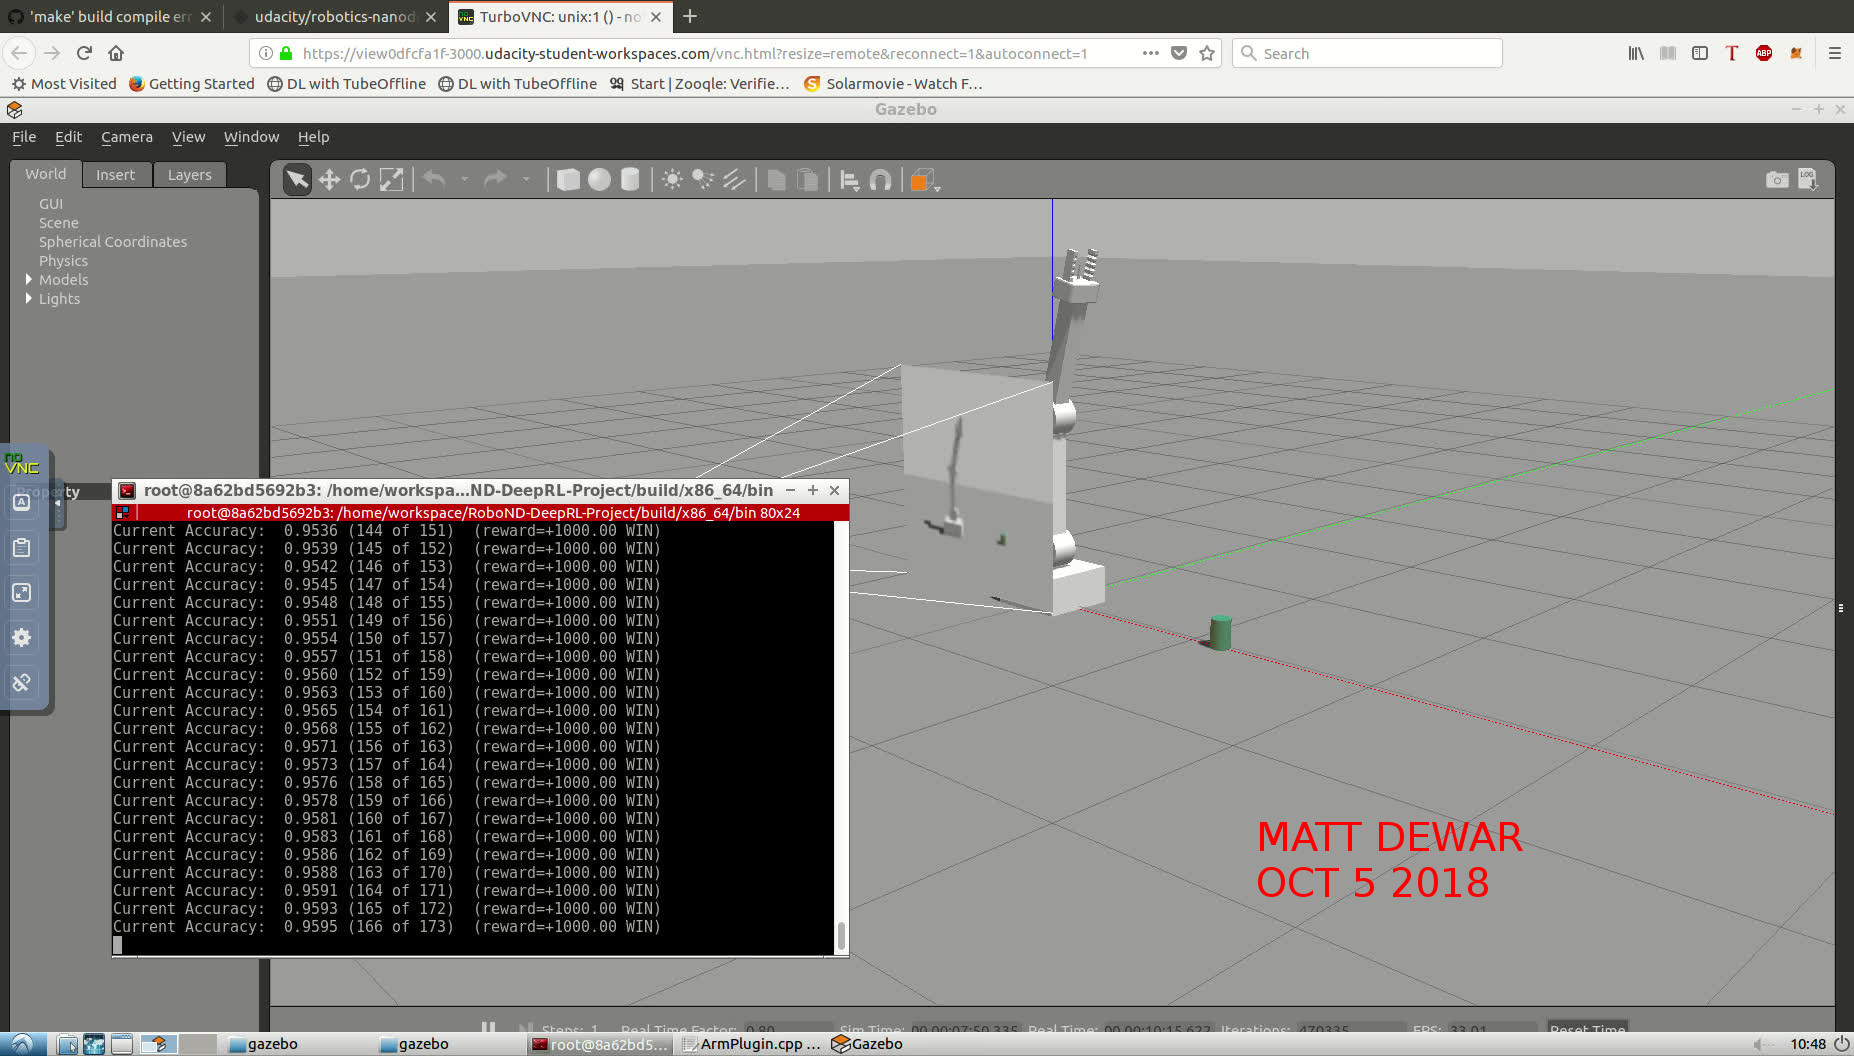
\includegraphics[width=\linewidth]{../images/Deep_RL-task1.jpg}
		\caption{Success rate for task 1 after 173 episodes.}
		\label{fig:task1}
	\end{figure}
	
	\subsection{Task 2}\label{subsec:task2}

	Training of the DQN agent was proven to be much more difficult in task 2, where initially the robot was observed to be hesitant to move forward towards the object after a significant amount of episodes, where a successful policy could not be found. Replay memory was first increased from 10000 to 20000 experience tuples in order to recall more experiences in the replay buffer. Being able to increase the randomization of experience tuples to choose from can help break state action correlation and actions values from diverging or oscillating \cite{UdacityLesson23}. However, with just this change the agent was unable to win an episode until episode 15, and took over 600 runs to get an accuracy of 80\%.

	The reward system was then decided to be modified leaving hyperparameters the same as in task 1, where an issued reward or penalty at the end of the episode would be proportional to the distance between the gripper and the object (Section. \ref{sec:rewards}). A proportional penalty in the case of the episode reaching the maximum timestep seemed to not help with training, compared to just setting the reward to the max win and max loss values. However it was found that if the robot's gripper is below a distance of 0.3 away from the object, and a proportional penalty is issued if the robot arm touches the part instead of the gripper, this reward system provides a great incentive that the chosen policy is on the right track. While an 80\% success rate was able to be achieved with this reward system it took the DQN agent 350 episodes to reach this, where an optimal policy was only being consistently chosen after 140 episodes of training. Results of this agent can be found in Figure. \ref{fig:task2}.

	\begin{figure}[thpb]
		\centering
		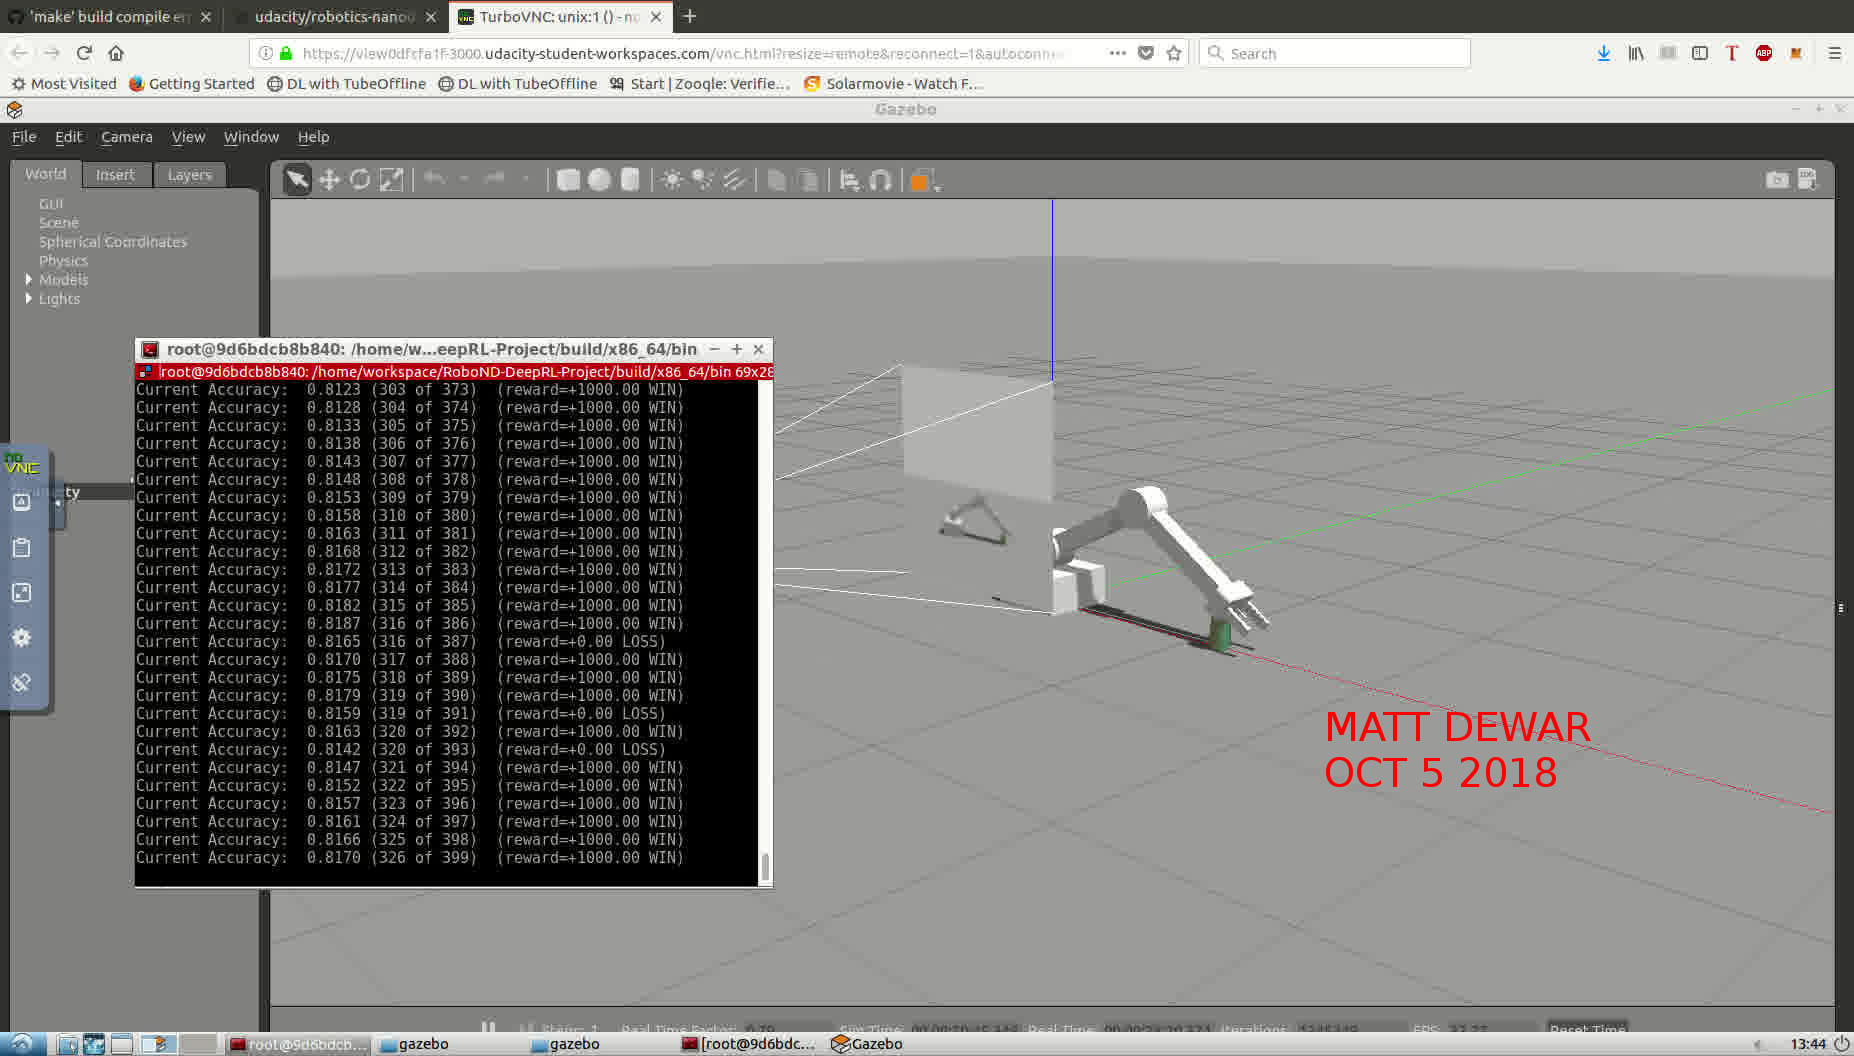
\includegraphics[width=\linewidth]{../images/Deep_RL-task2.jpg}
		\caption{Success rate for task 2 after 399 episodes.}
		\label{fig:task2}
	\end{figure}

	%%%%%%%%%%%%%%%%%%%%%%%%%%%%%%%%%%%%%%%%%%%%%%%%%%
%%%              CONCLUSIONS SECTION              %%%%
%%%%%%%%%%%%%%%%%%%%%%%%%%%%%%%%%%%%%%%%%%%%%%%%%%		

	\section{Future Work}\label{sec:future}
	Optimization of task 2 to achieve 80\% success in less than 300 episodes needs to be accomplished by retuning hyperparameters, or working out different reward strategies for the task. One such example would be to include incentive in touching the target as quick as possible. Exploring the velocity control system for task 2 may also be an encouraging venture. Experimenting with the epsilon greedy policy parameters should be done to evaluate policy training time in order to decrease the amount of episodes needed to arrive at an optimal policy for task 2. It is hypothesized that the epsilon greedy policy may be too exploratory, and may be the reason for taking so many episodes in order to achieve an 80\% success rate. Lastly, The extra challenges should be addressed, a DQN agent should be trained in actually picking up the object, and this project should be compiled and run on a Jetson TX2.

	
\section{References}
\bibliography{bib}   % .bib info
%%%%%%%%%%%%%%%%% Reference Style %%%%%%%%%%%%%%%%%%%
% Needs to be changed based on the journal you are sumbitting to. 
% see ``bst\journal_refstyles.pdf'' for more information
\bibliographystyle{bst/model3-num-names}		

\end{document}